\documentclass{standalone}
\usepackage{tikz}
\usepackage[]{xcolor}
\usetikzlibrary{calc}
\usepackage{bbold}
\usepackage{physics}

\newcommand{\mcG}{\mathcal{G}}

\graphicspath{{/}{../figs/}{/home/jadeleon/Documents/doctorado/2025-2/protocolo_candidatura/gfx/chaos/}}


\usepackage{amsmath, amsthm, amssymb}
\colorlet{coscolor}{blue}

\newcommand{\red}{\color{red}}
\newcommand{\blue}{\color{blue}}
%Colors

\definecolor{max}{rgb}{1,0.54,0.1}
\definecolor{medium}{rgb}{1,0.8,0.6}
\definecolor{min}{rgb}{1,0.9,0.8}
\begin{document}
\pagestyle{empty}
\newcommand{\tmpa}{6}
\newcommand{\tmpb}{4}
\newcommand{\xo}{0.5}
\newcommand{\separation}{0.97}
\newcommand{\scalefont}{1}
%meanLevelSpacing_distribution_chaotic
\begin{tikzpicture}
%\node[anchor=north west] at (\xo, 0.12) {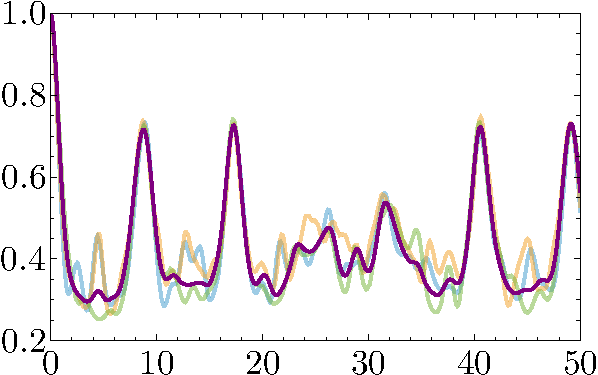
\includegraphics[height=3.63cm]{choi_regular_purity2.pdf}};
%\node[anchor=north west] at (\xo + \separation*\tmpa, 0)
%{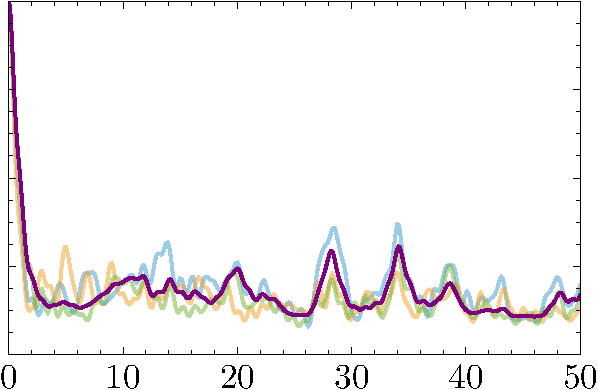
\includegraphics[height=3.5 cm]{choi_chaotic_purity2.pdf}};
%\fill[white] (\xo + 1.7*\separation*\tmpa, -1) rectangle (\xo + 1.95*\separation*\tmpa, -0.4);

%\fill[white] (0.7, -4) rectangle (1.01, -0.2);
%\node[rotate=90] at (0.3, -1.77) {$\Tr[\mathcal D^2(t)]$};
%\fill[white] (6.8, -4) rectangle (7.15, -0.2);
%\node[rotate=90] at (6.95, -1.77) {$\Tr[\mathcal D^2(t)]$};
%\fill[white] (3, -4.09) rectangle (5, -3.85);
%\fill[white] (10, -4.09) rectangle (12, -3.85);


%\node[anchor=north west] at (1.75, -0.15) {\scalebox{\scalefont}{(a)}};
%\node[anchor=north west] at (7.8, -0.15) {\scalebox{\scalefont}{(b)}};

%%%%%%%%%%%%%%%
\node[] at (1.7,2) {
\includegraphics[height=0.1cm]{legends.pdf}};
\node[] at (-0.8, 2) {$\Tr[\mathcal{D}(t)^2]$};
\node[] at (1.7, 2) {$\Tr[\mathcal{D}(t)^2]$};
\node[] at (4.1, 2) {$\Tr[\mathcal{D}(t)^2]$};
\node[] at (7.1,2) {$\ev{\Tr[\mathcal{D}(t)^2]}_{\mathrm{Haar}}$};

\begin{scope}[shift={(0,0)}]
\node[anchor=south west] at (-2.3, 1) {\scalebox{\scalefont}{(a)}};
\node[] at (0,0) {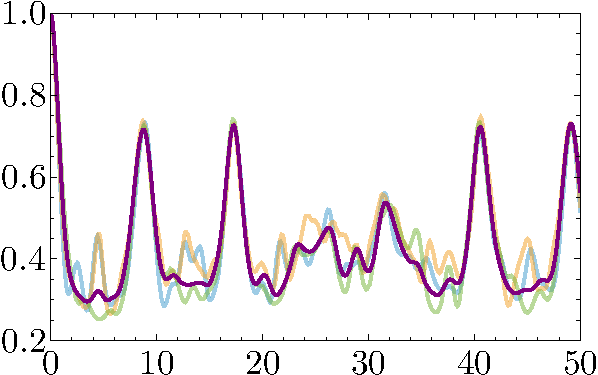
\includegraphics[height=3.65cm]{choi_regular_purity2.pdf}};
\node[anchor=south west] at (-0.67,0.05)
{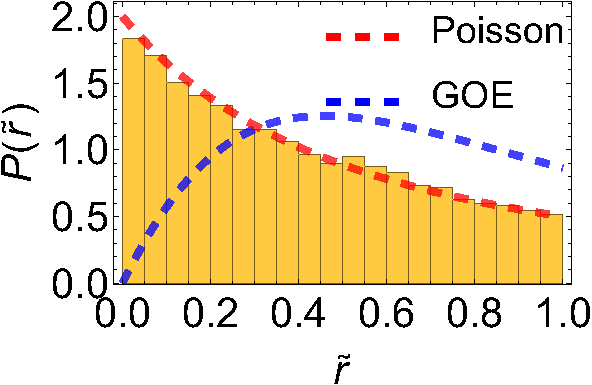
\includegraphics[height=1.42cm]{meanLevelSpacing_distribution_regular.pdf}};

\node at (0.2, -2) {$t$};
\end{scope}

\begin{scope}[shift={(5.75,-0.06)}]
\node[anchor=south west] at (-2.5, 1) {\scalebox{\scalefont}{(b)}};
\node[] at (0,0) {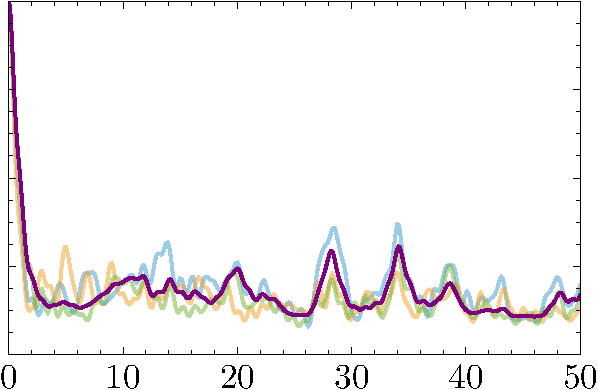
\includegraphics[height=3.5cm]{choi_chaotic_purity2.pdf}};
\node[anchor=south west] at (-0.67,0.05)
{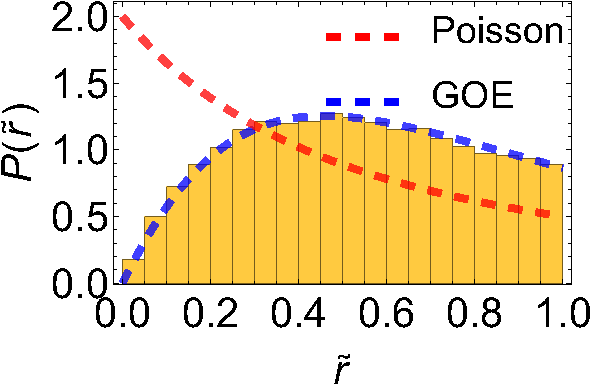
\includegraphics[height=1.42cm]{meanLevelSpacing_distribution_chaotic.pdf}};

\node at (0, -2) {$t$};
\end{scope}
\end{tikzpicture}
\end{document}